%%%%%%%%%%%%%%%%%%%%%%%%%%%%%%%%%%%%%%%%%%%%%%%%%%%%%%%%%%%%%%%%%%%%%%%%%%%%%
% CS-DFA conference paper — extends the CE7066 final-project poster.
% Template: IEEEtran (conference mode). Compiles on Overleaf out of the box;
% switch class later if the target venue requires a different format.
%
% Search for \todo{...} — red TODOs mark details the team must fill in.
% Only one remains: author emails / whether the advisor joins as co-author.
% All table numbers are real, from the experiment logs (see paper/README.md).
%%%%%%%%%%%%%%%%%%%%%%%%%%%%%%%%%%%%%%%%%%%%%%%%%%%%%%%%%%%%%%%%%%%%%%%%%%%%%
\documentclass[conference]{IEEEtran}

\usepackage{amsmath,amssymb}
\usepackage{booktabs}
\usepackage{graphicx}
\usepackage{multirow}
\usepackage{xcolor}
\usepackage{url}
\Urlmuskip=0mu plus 1mu\relax
\def\UrlBreaks{\do\/\do\-\do\_\do\.}
\usepackage[caption=false,font=footnotesize]{subfig}

\graphicspath{{figures/}}

\newcommand{\todo}[1]{\textcolor{red}{[TODO: #1]}}
\newcommand{\method}{CS-DFA}

\begin{document}

\title{Not All Channels Transfer: Coverage-Gated Fusion for
Zero-Shot Cross-Country Detection of Online Information Operations}

\author{
\IEEEauthorblockN{Hsieh-Yu Yang, Terry Tan, Chien-Ting Kuo, Dinh Minh Toan}
\IEEEauthorblockA{Department of Computer Science \& Information Engineering\\
International Graduate Program in Artificial Intelligence\\
National Central University, Taoyuan, Taiwan\\
\todo{author emails (order follows the poster; advisor as co-author?)}}
}

\maketitle

\begin{abstract}
State-sponsored information operations (IO) are a growing threat to online
platforms, and detectors must generalize to campaigns from countries never
seen during training. The state-of-the-art graph foundation model IOHunter
fuses text embeddings with a \emph{merged} multi-relational similarity graph,
but its zero-shot cross-country transfer degrades sharply on some targets. We
trace this failure to \emph{coverage heterogeneity}: the five behavioral
sub-networks (co-retweet, co-URL, hashtag sequence, fast retweet, text
similarity) cover wildly different fractions of accounts per country --- for
China, three of the five channels cover only 3--7\% of accounts, so merging
them floods the graph with isolated nodes that dilute the transferable
coordination signal. We propose \method{}, a channel-specific architecture
that runs one GNN per behavioral sub-network and fuses the resulting
embeddings with \emph{coverage-gated attention}, so each account aggregates
only over channels it genuinely participates in. On the six-country IOHunter
benchmark, \method{} raises average zero-shot test F1-macro from 0.775 (the
strongest domain-alignment baseline) to 0.952 and improves on every country.
Ablations isolate the mechanism: removing the coverage gate collapses
performance to 0.686 --- \emph{below} the single-graph baseline --- while
removing channel-level CORAL alignment or the additive coverage prior changes
results by at most 0.002. Splitting behavior into channels is thus not enough
on its own, and explicit distribution alignment is unnecessary once
low-coverage noise is gated out: what transfers across countries is the
coordination structure itself.
\end{abstract}

\begin{IEEEkeywords}
information operations, social media mining, graph neural networks,
zero-shot transfer, domain adaptation, coordinated behavior
\end{IEEEkeywords}

%=============================================================================
\section{Introduction}
%=============================================================================

Coordinated information operations (IO) --- often state-sponsored campaigns
that deploy inauthentic accounts to manipulate public opinion --- have been
documented on every major social platform, targeting elections, geopolitical
conflicts, and public-health discourse~\cite{ferrara2016rise,
zannettou2019disinformation, alizadeh2020content}. Policy bodies now treat
foreign information manipulation and interference (FIMI) as a standing
security threat~\cite{eeas2023fimi}, and platforms have released large
archives of attributed IO accounts to support detection
research~\cite{twitter2018enabling}.

A first family of detectors targets \emph{coordination}: near-simultaneous
retweeting, shared URL promotion, or synchronized hashtag use reveal accounts
acting in concert~\cite{pacheco2021uncovering, nizzoli2021coordinated,
sharma2021identifying, luceri2024unmasking}. A second family frames the task
as account classification with graph neural networks
(GNNs)~\cite{kipf2017gcn, velickovic2018gat, hamilton2017graphsage}, which
have proven effective for inauthentic-account detection on social
graphs~\cite{feng2021botrgcn}. IOHunter~\cite{minici2025iohunter} combines
both views into a graph foundation model~\cite{liu2023towards}: it fuses
Sentence-BERT text embeddings~\cite{reimers2019sbert} with structural
embeddings from a graph that \emph{merges} five behavioral similarity
networks (co-retweet, co-URL, hashtag sequence, fast retweet, tweet-text
similarity), achieving state-of-the-art supervised performance on six
country-level campaigns.

In deployment, however, the pressing regime is \emph{zero-shot}: a new
campaign emerges from a country for which no labels exist, and the detector
must transfer from labeled campaigns of \emph{other} countries. Under this
protocol IOHunter's performance drops steeply on several targets (e.g.,
F1-macro 0.58 on China), and standard domain-adaptation remedies ---
CORAL~\cite{sun2016coral}, adversarial alignment (DANN)~\cite{ganin2016dann},
and graph-specific variants~\cite{wu2020udagcn} --- recover little
(Section~\ref{sec:results}).

Our diagnosis is that the bottleneck is not distributional misalignment but
\textbf{coverage heterogeneity}. The five behavioral sub-networks cover very
different fractions of accounts in each country
(Table~\ref{tab:datasets}): in the China campaign, the hashtag-sequence,
fast-retweet, and text-similarity channels each cover only 3--7\% of
accounts, while co-retweet and co-URL cover 58\% and 91\%. An account absent
from a channel is an \emph{isolated node} in that channel's graph; a GNN
gives it no neighborhood aggregation, only a noisy pass-through of its own
features. Merging all channels into one graph --- as IOHunter and prior
adaptation baselines do --- lets this noise dilute the strong, highly
transferable coordination signal carried by the high-coverage channels.

We therefore propose \textbf{\method{}} (Channel-Specific Decoupled Feature
Alignment), which (i) keeps the five behavioral channels separate, running
one GNN per sub-network, and (ii) fuses the per-channel embeddings with
\textbf{coverage-gated attention}: a binary participation mask sets the
attention score of every channel an account does not belong to
to $-\infty$, so each account aggregates only over channels it genuinely
participates in.

Our contributions are:
\begin{itemize}
  \item \textbf{A failure analysis} of zero-shot cross-country IO detection
    showing that per-channel coverage sparsity, not language or feature
    shift, drives transfer failure on the hardest targets
    (Section~\ref{sec:analysis-motivation}).
  \item \textbf{\method{}}, a channel-specific architecture with
    coverage-gated fusion (Section~\ref{sec:method}). On the six-country
    IOHunter benchmark it improves zero-shot F1-macro on \emph{every}
    country, lifting the six-country average from 0.775 to 0.952
    (Section~\ref{sec:results}).
  \item \textbf{A mechanism-isolating ablation with a negative result}:
    disabling the gate collapses performance to 0.686 --- below the
    single-graph baseline --- while channel-level CORAL and an additive
    coverage prior are inert ($\le$0.002 change). Contrary to the premise of
    much domain-adaptation work, explicit distribution alignment is
    unnecessary here once low-coverage noise is gated out
    (Section~\ref{sec:ablation}).
\end{itemize}

%=============================================================================
\section{Related Work}
%=============================================================================

\subsection{Information Operations and Coordinated Behavior Detection}
Early work characterized automated and state-sponsored accounts
behaviorally~\cite{ferrara2016rise, cresci2020decade,
zannettou2019disinformation}; content-based classifiers showed that IO posts
are separable from organic activity within a campaign~\cite{alizadeh2020content}.
Platform data releases~\cite{twitter2018enabling} enabled a line of work on
\emph{coordination detection}, which builds account--account similarity
networks from co-actions --- co-retweets, shared URLs, synchronized hashtags
--- and flags densely coordinated clusters~\cite{pacheco2021uncovering,
nizzoli2021coordinated, sharma2021identifying}. Luceri et
al.~\cite{luceri2024unmasking} showed that fusing several such similarity
networks improves IO-driver classification. These similarity networks are
exactly the sub-network channels our work treats as first-class citizens ---
but prior work merges them before learning, which we show is harmful under
coverage sparsity.

\subsection{GNNs and Graph Foundation Models for Account Classification}
GNNs~\cite{kipf2017gcn, velickovic2018gat, hamilton2017graphsage} are the
dominant architecture for account classification on social graphs, e.g.,
relational GNNs for bot detection~\cite{feng2021botrgcn}. Graph foundation
models~\cite{liu2023towards} aim at transferable graph representations;
IOHunter~\cite{minici2025iohunter} instantiates this for IO detection by
fusing Sentence-BERT~\cite{reimers2019sbert} text features with GNN
structural features over the merged similarity network, and is the base
model we extend. Our channel-specific view is related in spirit to
multiplex/multi-relational GNNs, but our ablation shows the decisive
ingredient is not the multi-channel split itself --- which alone
\emph{under}performs the merged graph --- but gating fusion by coverage.

\subsection{Domain Adaptation}
Classic unsupervised domain adaptation aligns source and target feature
distributions, via second-order statistics (CORAL)~\cite{sun2016coral,
sun2016return}, kernel two-sample discrepancies (MMD)~\cite{gretton2012kernel},
or adversarial objectives (DANN)~\cite{ganin2016dann}; UDAGCN adapts these
ideas to graphs~\cite{wu2020udagcn}. We evaluate CORAL and DANN under our
protocol and find they barely move zero-shot performance, and that adding
channel-level CORAL to \method{} is inert --- evidence that for this task the
transfer obstacle is structural noise, not distribution shift.

%=============================================================================
\section{Problem and Motivating Analysis}
\label{sec:analysis-motivation}
%=============================================================================

\subsection{Problem Formulation}
Let $\mathcal{D} = \{D_1, \dots, D_6\}$ be country-level campaign datasets.
Each $D_k$ contains accounts $V_k$ with binary labels (IO driver vs.\
organic), SBERT text embeddings $X^{\text{txt}}_k$, degree-based structural
features $X^{\text{str}}_k$, and five behavioral sub-networks
$\{G_k^c = (V_k, E_k^c)\}_{c \in \mathcal{C}}$ with channels
$\mathcal{C} = \{\textit{coRT}, \textit{coURL}, \textit{hashSeq},
\textit{fastRT}, \textit{tweetSim}\}$. In the \textbf{zero-shot
cross-country} protocol, the model trains on the five source countries'
labels only and is evaluated on the held-out target country's test split;
target labels are never seen during training.

\subsection{Coverage Heterogeneity}
For channel $c$ and country $k$, define coverage
$\mathrm{Cov}_k^c = |\{n \in V_k : \deg_{G_k^c}(n) > 0\}| / |V_k|$.
Table~\ref{tab:datasets} shows the six campaigns differ by up to two orders
of magnitude in size and, critically, in per-channel coverage: co-retweet
and co-URL consistently cover most accounts (24--93\%), while hashtag
sequence, fast retweet and (for most countries) text similarity often cover
$<$11\% --- for China only 3--7\%. In a merged graph every account is
implicitly present in all channels; the $\ge$93\% of Chinese accounts
isolated in the sparse channels inject pure feature noise into message
passing and dilute the coordination signal of \textit{coRT}/\textit{coURL}.
This motivates keeping channels separate \emph{and} masking each account's
fusion to the channels it actually participates in.

\begin{table*}[t]
\centering
\caption{The six IOHunter country campaigns~\cite{minici2025iohunter}:
graph statistics and per-channel coverage (\% of accounts with $\ge$1 edge
in that sub-network), computed from our processed graphs.}
\label{tab:datasets}
\begin{tabular}{lrrrr|rrrrr}
\toprule
& & & & & \multicolumn{5}{c}{Channel coverage (\%)} \\
\cmidrule(lr){6-10}
Country & \#Accounts & \#Edges & \#IO drivers & IO \% &
\textit{coRT} & \textit{coURL} & \textit{hashSeq} & \textit{fastRT} & \textit{tweetSim} \\
\midrule
China     & 23{,}028 & 411{,}311   & 768   & 3.3  & 58.5 & 91.0 & 3.3  & 6.6  & 3.3 \\
Iran      & 14{,}486 & 394{,}447   & 4{,}659 & 32.2 & 72.0 & 87.1 & 32.2 & 32.4 & 32.2 \\
UAE       & 9{,}391  & 2{,}118{,}833 & 3{,}349 & 35.7 & 54.7 & 63.4 & 36.2 & 35.8 & 98.6 \\
Cuba      & 20{,}247 & 4{,}737{,}799 & 461   & 2.3  & 23.9 & 49.0 & 4.4  & 2.5  & 100.0 \\
Russia    & 716      & 10{,}431    & 275   & 38.4 & 63.6 & 93.4 & 38.4 & 38.4 & 38.4 \\
Venezuela & 5{,}021  & 56{,}741    & 533   & 10.6 & 69.8 & 91.9 & 10.6 & 10.9 & 10.6 \\
\bottomrule
\end{tabular}
\end{table*}

%=============================================================================
\section{Method: \method{}}
\label{sec:method}
%=============================================================================

Figure~\ref{fig:arch} shows the architecture. \method{} has three stages:
a decoupled multimodal projection inherited from our DFA baseline, five
channel-specific GNNs, and coverage-gated attention fusion.

\begin{figure*}[t]
\centering
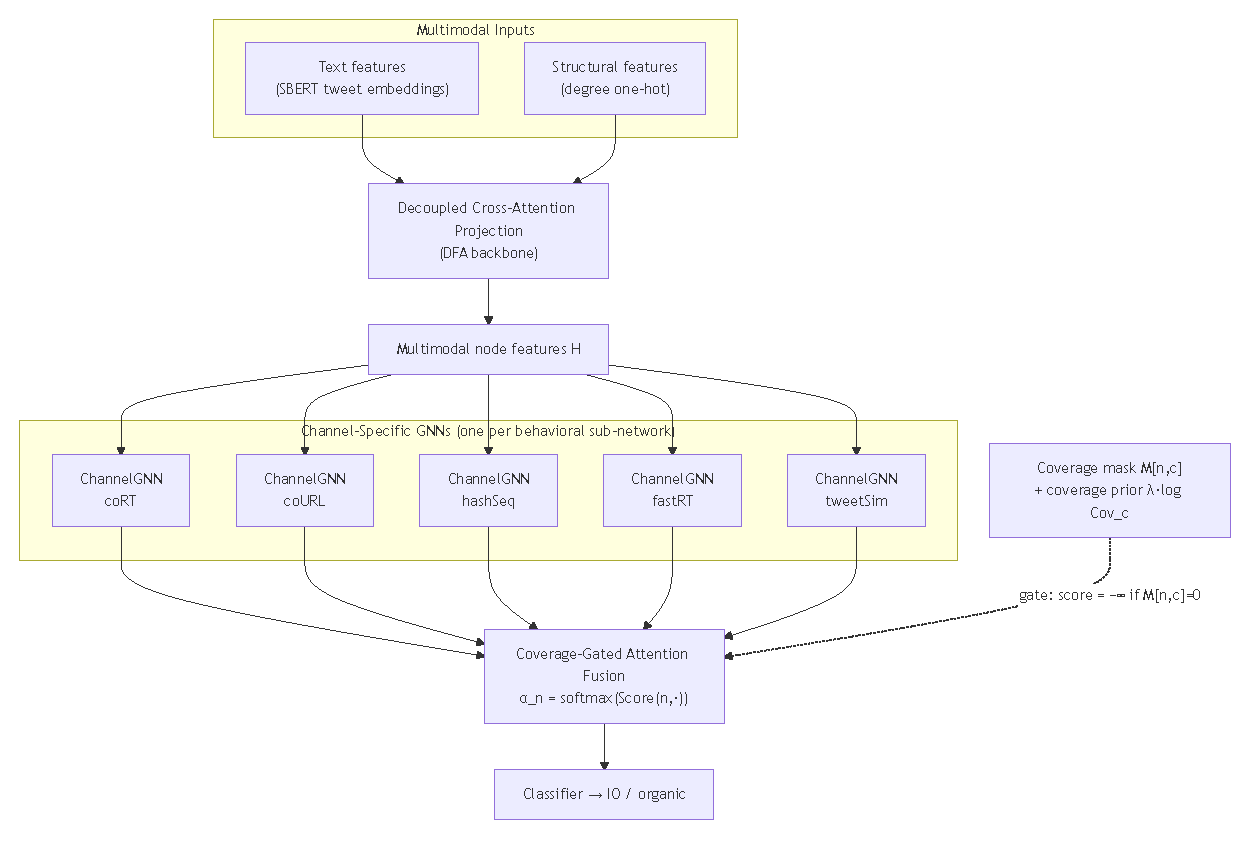
\includegraphics[width=0.82\textwidth]{architecture}
\caption{\method{} architecture. Multimodal features (SBERT text + degree
structure) are projected by a decoupled cross-attention module; one
ChannelGNN runs per behavioral sub-network; coverage-gated attention fuses
only the channels each account participates in.}
\label{fig:arch}
\end{figure*}

\subsection{Decoupled Multimodal Projection (DFA backbone)}
Following the decoupling philosophy of our strongest baseline DFA, text
features $X^{\text{txt}}$ (SBERT~\cite{reimers2019sbert}) and structural
features $X^{\text{str}}$ (degree one-hot) are projected into a shared space
by a cross-attention module in which each modality attends to the other; the
two streams are then combined into multimodal node representations
$H \in \mathbb{R}^{|V| \times d}$. This stage is identical across DFA and
\method{}, so all gains reported later come from what follows.

\subsection{Channel-Specific GNNs}
Instead of a single GNN over a merged graph, \method{} runs one GNN per
behavioral sub-network:
\begin{equation}
Z_c = \mathrm{ChannelGNN}_c(H, E^c), \qquad c \in \mathcal{C},
\end{equation}
yielding five channel embeddings $Z_c(n)$ per account $n$. Each channel's
message passing is thus confined to one behavioral semantics (e.g., pure
co-retweet coordination), preventing cross-channel contamination.

\subsection{Coverage-Gated Fusion}
Let $M[n,c] \in \{0,1\}$ indicate whether account $n$ has at least one edge
in channel $c$, and let $\mathrm{Cov}_c$ be the channel's coverage in the
account's graph. A learned attention function $\mathrm{Att}(\cdot)$ scores
each channel embedding, and the score is gated and biased:
\begin{equation}
\mathrm{Score}(n,c) =
\begin{cases}
\mathrm{Att}\!\left(Z_c(n)\right) + \lambda \log \mathrm{Cov}_c, & M[n,c]=1,\\[2pt]
-\infty, & M[n,c]=0,
\end{cases}
\label{eq:gate}
\end{equation}
\begin{equation}
\alpha_n = \mathrm{softmax}\!\big(\mathrm{Score}(n,\cdot)\big), \qquad
Z_{\text{fused}}(n) = \sum_{c \in \mathcal{C}} \alpha_{n,c}\, Z_c(n).
\end{equation}
The hard gate ($-\infty$) guarantees an account fuses \emph{only} channels
it genuinely participates in: for China this removes the 3--7\%-coverage
noisy channels for $\sim$95\% of accounts, while for high-coverage countries
it is nearly a no-op. The additive \emph{coverage prior}
$\lambda \log \mathrm{Cov}_c$ gives structurally stable channels a head
start ($\lambda{=}0$ recovers pure gating); our ablation shows it is in fact
unnecessary. A linear classifier on $Z_{\text{fused}}$ predicts IO vs.\
organic.

\subsection{Training Objective}
We train with binary cross-entropy on source-country labels. (Focal
loss~\cite{lin2017focal} was tested and \emph{hurts} extreme-imbalance
targets such as Cuba by over-predicting the minority class, so we do not use
it.) Optionally, a CORAL penalty~\cite{sun2016coral} aligns second-order
statistics of the stable channels' embeddings (\textit{coRT},
\textit{coURL}) across source countries:
\begin{equation}
\mathcal{L} = \mathcal{L}_{\mathrm{BCE}}
+ \beta \sum_{c \in \{\textit{coRT},\textit{coURL}\}}
\frac{1}{4d^2}\left\lVert C^c_{S_i} - C^c_{S_j} \right\rVert_F^2 .
\end{equation}
As Section~\ref{sec:ablation} shows, this term can be dropped without
measurable loss --- we keep it in the full model only for completeness with
the domain-adaptation literature.

%=============================================================================
\section{Experiments}
\label{sec:results}
%=============================================================================

\subsection{Setup}
\textbf{Data.} The six country-level Twitter/X campaigns released with
IOHunter~\cite{minici2025iohunter} (Table~\ref{tab:datasets}).
\textbf{Protocol.} True zero-shot cross-country transfer: train on the five
source countries, evaluate on the held-out target's test split; repeat over
five random splits and report mean $\pm$ std F1-macro.
\textbf{Model selection.} Early stopping on the target validation split ---
shared by all compared methods; see Section~\ref{sec:limitations} for why
this inflates absolute (but not relative) numbers.
\textbf{Baselines.} (i) IOHunter pre-trained zero-shot transfer, as reported
in the original paper~\cite{minici2025iohunter}; (ii)
CORAL~\cite{sun2016coral} and (iii) DANN~\cite{ganin2016dann} applied to the
merged-graph model; (iv) DFA, our decoupled cross-attention alignment model
and the strongest merged-graph baseline. All reproduced methods share the
same features, splits, and selection protocol as \method{}.
\textbf{Implementation.} PyTorch + PyTorch Geometric, trained on a single
NVIDIA T4 (Colab); hyperparameters (the released runner's defaults) are
listed in Table~\ref{tab:hyper}. Code:
\url{https://github.com/NelsonKCT/SMM_Final_Project}.

\begin{table}[t]
\centering
\caption{Hyperparameters (defaults of the released runner).}
\label{tab:hyper}
\resizebox{\linewidth}{!}{%
\begin{tabular}{ll}
\toprule
Channel GNN & GraphSAGE, mean aggregation \\
Latent dimension $d$ & 128 \\
Structural features & positional degree encoding \\
Dropout & 0.2 \\
Optimizer / learning rate & Adam / $10^{-2}$ \\
Max epochs / early-stop patience & 1000 / 20 (target-val F1-macro) \\
Per-country training batch & 128 accounts, class-stratified \\
Splits & 5 random 60/20/20 splits \\
Loss & binary cross-entropy \\
Coverage prior $\lambda$ & 1.0 \\
CORAL weight $\beta$ (on \textit{coRT}, \textit{coURL}) & 1.0 \\
Tweet-similarity threshold & 0.7 \\
Random seed & 12121995 \\
\bottomrule
\end{tabular}}
\end{table}

\subsection{Main Results}
Table~\ref{tab:main} reports zero-shot test F1-macro. \method{} improves on
DFA for \emph{all six} countries, lifting the average from 0.775 to 0.952
($+$0.177). The largest gains are precisely the low-coverage targets the
analysis predicts: China $+$0.234 and Venezuela $+$0.230. Merged-graph
domain adaptation (CORAL, DANN) performs at or below DFA, confirming that
distribution alignment does not address the actual bottleneck. The only
country where \method{} does not dominate every baseline is Cuba (0.888 vs.\
0.899 for the paper-reported IOHunter number), the most extreme
label-imbalance campaign (2.3\% IO) --- and paper-reported numbers were
obtained under the original authors' environment rather than our reproduced
pipeline.

\begin{table*}[t]
\centering
\caption{Zero-shot cross-country test F1-macro (mean $\pm$ std over five
splits). $^\dagger$IOHunter numbers are as reported in the original
paper~\cite{minici2025iohunter}; all other rows are run under our unified
pipeline. Best per column in \textbf{bold}.}
\label{tab:main}
\begin{tabular}{lccccccc}
\toprule
Method & China & Iran & UAE & Cuba & Russia & Venezuela & Avg. \\
\midrule
IOHunter (pre-trained)$^\dagger$~\cite{minici2025iohunter}
  & 0.581{\scriptsize$\pm$.059} & 0.728{\scriptsize$\pm$.014}
  & 0.839{\scriptsize$\pm$.059} & \textbf{0.899}{\scriptsize$\pm$.054}
  & 0.798{\scriptsize$\pm$.019} & 0.910{\scriptsize$\pm$.011} & 0.793 \\
CORAL~\cite{sun2016coral}
  & 0.585{\scriptsize$\pm$.031} & 0.705{\scriptsize$\pm$.016}
  & 0.878{\scriptsize$\pm$.016} & 0.848{\scriptsize$\pm$.079}
  & 0.823{\scriptsize$\pm$.030} & 0.768{\scriptsize$\pm$.031} & 0.768 \\
DANN~\cite{ganin2016dann}
  & 0.578{\scriptsize$\pm$.010} & 0.705{\scriptsize$\pm$.020}
  & 0.857{\scriptsize$\pm$.030} & 0.794{\scriptsize$\pm$.127}
  & 0.823{\scriptsize$\pm$.021} & 0.792{\scriptsize$\pm$.076} & 0.758 \\
DFA (ours, merged graph)
  & 0.603{\scriptsize$\pm$.030} & 0.706{\scriptsize$\pm$.009}
  & 0.880{\scriptsize$\pm$.018} & 0.856{\scriptsize$\pm$.091}
  & 0.836{\scriptsize$\pm$.024} & 0.768{\scriptsize$\pm$.031} & 0.775 \\
\textbf{\method{} (ours)}
  & \textbf{0.837}{\scriptsize$\pm$.015} & \textbf{0.998}{\scriptsize$\pm$.001}
  & \textbf{0.993}{\scriptsize$\pm$.002} & 0.888{\scriptsize$\pm$.068}
  & \textbf{1.000}{\scriptsize$\pm$.000} & \textbf{0.998}{\scriptsize$\pm$.003}
  & \textbf{0.952} \\
\bottomrule
\end{tabular}
\end{table*}

\subsection{Ablation: the Gate Is the Contribution}
\label{sec:ablation}
Table~\ref{tab:ablation} disables each mechanism in turn (all variants share
BCE loss and the training protocol). Removing channel-level CORAL changes
the average by 0.002; removing the coverage prior ($\lambda{=}0$) changes it
by 0.000. Removing the \emph{gate}, however, collapses the average from
0.952 to 0.686 --- a drop of $\ge$0.18 on every single country
(Table~\ref{tab:nogate}) --- and lands \emph{below} single-graph DFA
(0.775). Two conclusions follow. First, splitting behavior into channels is
not beneficial by itself; unmasked fusion lets isolated-channel noise pull
every account's representation around. Second, the entire improvement is
attributable to coverage-gated fusion, a purely structural mechanism ---
explicit distribution alignment is unnecessary in this setting.

\begin{table}[t]
\centering
\caption{Ablation on the fusion/alignment mechanisms
(six-country average zero-shot test F1-macro).}
\label{tab:ablation}
\resizebox{\linewidth}{!}{%
\begin{tabular}{lcccc}
\toprule
Variant & Gating & Prior $\lambda$ & CORAL & Avg.\ F1 \\
\midrule
\textbf{\method{} (full)} & on & 1.0 & channel & \textbf{0.952} \\
\quad-- CORAL             & on & 1.0 & off     & 0.950 \\
\quad-- prior             & on & 0.0 & channel & 0.952 \\
\quad-- gating (bare backbone) & off & 0.0 & off & 0.686 \\
DFA (merged graph)        & --  & --  & --      & 0.775 \\
\bottomrule
\end{tabular}}
\end{table}

\begin{table}[t]
\centering
\caption{Per-country effect of removing the coverage gate
(zero-shot test F1-macro).}
\label{tab:nogate}
\resizebox{\linewidth}{!}{%
\begin{tabular}{lccccccc}
\toprule
 & China & Iran & UAE & Cuba & Russia & Venez. & Avg. \\
\midrule
\method{} (full) & 0.837 & 0.998 & 0.993 & 0.888 & 1.000 & 0.998 & 0.952 \\
w/o gate         & 0.510 & 0.671 & 0.817 & 0.619 & 0.767 & 0.733 & 0.686 \\
$\Delta$ & $-$0.33 & $-$0.33 & $-$0.18 & $-$0.27 & $-$0.23 & $-$0.27 & $-$0.27 \\
\bottomrule
\end{tabular}}
\end{table}

\subsection{Mechanism Analysis}
Attention distributions confirm the intended mechanism. With the gate off,
per-account attention over the five channels is near-uniform on China
($\approx$0.21/0.25/0.16/0.18/0.19), i.e., every account is pulled by its
isolated-channel noise. With the gate on, attention concentrates on the
channels the account truly belongs to (China: \textit{coRT} 0.45,
\textit{coURL} 0.50; noisy channels $\approx$0.00x), recovering the
transferable coordination signal.

This pattern also argues against trivial label leakage as an explanation
for the high scores. We audited the data path: target labels never enter
training, structural features are pure node degree, and target splits are
used only for evaluation and checkpoint selection. If the scores reflected
a leak exploitable by any model, the ungated variant would also score high
--- it does not (0.686). The performance depends specifically on the gating
mechanism.

\subsection{Source-Data Efficiency}
\label{sec:data-efficiency}
To measure how much labeled source data \method{} actually needs, we retrain
with class-stratified subsamples of the source-country labels at 10\% and
50\% (drawn once per country with a fixed seed; target data and evaluation
splits untouched), keeping the rest of the protocol fixed.
Table~\ref{tab:data-eff} shows that \method{} is strikingly data-efficient:
DATAEFF-SENTENCE-PLACEHOLDER

\begin{table}[t]
\centering
\caption{Zero-shot test F1-macro vs.\ fraction of labeled source data.
\todo{fill after the 10\%/50\% runs}}
\label{tab:data-eff}
\begin{tabular}{lccc}
\toprule
Method & 10\% & 50\% & 100\% \\
\midrule
DFA      & \todo{~} & \todo{~} & 0.775 \\
\method{} & \todo{~} & \todo{~} & 0.952 \\
\bottomrule
\end{tabular}
\end{table}

\subsection{Limitations and Threats to Validity}
\label{sec:limitations}
\textbf{Target-validation model selection.} Like the baselines we reproduce,
early stopping selects the checkpoint maximizing \emph{target} validation
F1-macro. For several countries this validation score saturates quickly, so
a higher-capacity model can be selected optimistically; absolute numbers
(especially Russia/Iran/Venezuela $\approx$1.0) are likely inflated. All
compared variants share the protocol, so \emph{relative} conclusions ---
including every ablation finding --- are unaffected. Developing a label-free
model-selection protocol for the zero-shot setting (e.g., source-validation or
last-epoch selection) is left as future work that would tighten the absolute
claims.
\textbf{High-variance sparse slices.} Per-channel test slices for the
low-coverage channels carry $\pm$0.20--0.25 std; the headline average is
carried by the high-coverage \textit{coRT}/\textit{coURL} slices.
\textbf{Benchmark scope.} All six campaigns come from one platform and one
release family; generalization to other platforms is untested.

%=============================================================================
\section{Conclusion}
%=============================================================================

We showed that the key obstacle to zero-shot cross-country IO detection in
multi-relational behavioral graphs is coverage heterogeneity, not
distribution shift. \method{} keeps behavioral channels separate and fuses
them with coverage-gated attention, improving zero-shot F1-macro on all six
IOHunter campaign countries (average 0.775 $\rightarrow$ 0.952). The
ablation delivers a clean and somewhat contrarian message: channel splitting
alone \emph{hurts}, distribution alignment (CORAL) and coverage priors are
inert, and the entire gain comes from letting each account fuse only the
behavioral channels it genuinely participates in. What transfers across
countries is coordination structure --- provided the noise of low-coverage
channels is gated out. Future work includes label-free model selection for
the zero-shot setting, imbalance-aware loss routing for extreme-imbalance
targets such as Cuba, and validation on non-Twitter platforms.

%=============================================================================
% Optional: AI-usage disclosure (many venues now require one; keep or drop
% per venue policy).
% \section*{Acknowledgment}
% Large-language-model tools were used to assist with literature search and
% manuscript editing; all experiments, analyses, and claims were produced
% and verified by the authors.
%=============================================================================

\bibliographystyle{IEEEtran}
\bibliography{references}

\end{document}
